%% ※このファイルを修正してください※

%% 産業技術大学院大学紀要LaTeXスタイルシート
%% Y.Chubachi 2012

%% jsarticleスタイルとmulticolを組み合わせて組版します
%% jsclasses -> http://www.misojiro.t.u-tokyo.ac.jp/suribt/jsclasses.pdf
%% ※このファイルは修正しないでください※

%% TODO: 和文の標題と著者名を表示しない方法

\documentclass[a4j,9pt,twoside]{jsarticle}
%%%%%%%%%%%%%%%%%%%%%%%%%%%%%%%%%%%%%%%%%%%%%%%%%%%%%%%%
%% パッケージ
%%%%%%%%%%%%%%%%%%%%%%%%%%%%%%%%%%%%%%%%%%%%%%%%%%%%%%%%
\usepackage{multicol} % 2段組み用(必須)

%%%%%%%%%%%%%%%%%%%%%%%%%%%%%%%%%%%%%%%%%%%%%%%%%%%%%%%%
%% ページのサイズ
%%%%%%%%%%%%%%%%%%%%%%%%%%%%%%%%%%%%%%%%%%%%%%%%%%%%%%%%
% 左右マージン
\setlength{\oddsidemargin}{-1.4mm}    % 標準(1in=25.4mm) -1.4mm = 24.0mm
\setlength{\evensidemargin}{-5.4mm}   % 標準(1in=25.4mm) -5.4mm = 20.0mm
% 上下マージン
\setlength{\topmargin}{4.6mm}         % 標準(1in=25.4mm) +4.6mm = 30.0mm
\setlength{\headheight}{0.0mm}
\setlength{\headsep}{0.0mm}
% テキストの大きさ
% (jsarticleで9pt指定のため長さの単位にtruemmを使っています)
\setlength{\textwidth}{166.0truemm}   % A4横210.0mm -(24.0+20.0)mm = 166.0mm
\setlength{\textheight}{247.0truemm}  % A4縦297mm - (20.0 + 30.0)mm =247.0mm

  
%%%%%%%%%%%%%%%%%%%%%%%%%%%%%%%%%%%%%%%%%%%%%%%%%%%%%%%%
%% 明朝体イタリックフォントに関する警告の抑制
%%%%%%%%%%%%%%%%%%%%%%%%%%%%%%%%%%%%%%%%%%%%%%%%%%%%%%%%
\DeclareFontShape{JY1}{mc}{m}{it}{<5> <6> <7> <8> <9> <10> sgen*min
    <10.95><12><14.4><17.28><20.74><24.88> min10 <-> min10}{}
\DeclareFontShape{JT1}{mc}{m}{it}{<5> <6> <7> <8> <9> <10> sgen*tmin
    <10.95><12><14.4><17.28><20.74><24.88> tmin10 <-> tmin10}{}

%%%%%%%%%%%%%%%%%%%%%%%%%%%%%%%%%%%%%%%%%%%%%%%%%%%%%%%%
%% タイトルの定義
%%%%%%%%%%%%%%%%%%%%%%%%%%%%%%%%%%%%%%%%%%%%%%%%%%%%%%%%
\makeatletter% @記号を通常文字として扱う
\newcommand*{\etitle}[1]{\gdef\@etitle{#1}}
\newcommand*{\eauthor}[1]{\gdef\@eauthor{#1}}
\newcommand*{\eabstract}[1]{\long\def\@eabstract{#1}}
\newcommand*{\keywords}[1]{\gdef\@keywords{#1}}
% http://ea3pch.yz.yamagata-u.ac.jp/member/sumio/tex/styleuse.pdf
\renewcommand{\maketitle}{%
  %\newpage\null
  %\vskip 2em
  \begin{center}
    \let\footnote\thanks
    % 和文標題
    {\LARGE \@title \par}%
    \vskip 1.5em
    {\large \@author \par}
    \vskip 2em
    % 英文標題
    {\Large\bf \@etitle \par}%
    \vskip 1em
    {\large\bf \@eauthor \par}%
    \vskip 2em
    % 英文概要
    {\large\bf Abstract}
  \end{center}%
  %\begin{quotation}
    {\normalsize \@eabstract \par}
  %\end{quotation}
  \vskip 1em
  {\normalsize {\bf Keywords:} \@keywords \par} 
  \vskip 1.5em
  \setcounter{footnote}{0}%
  \global\let\thanks\relax
  \global\let\maketitle\relax
  \global\let\@thanks\@empty
  \global\let\@title\@empty
  \global\let\@author\@empty
  \global\let\@etitle\@empty
  \global\let\@date\@empty
  \global\let\title\relax
  \global\let\author\relax
  \global\let\date\relax
  \global\let\and\relax
}%
\makeatother%  @記号を特殊文字に戻す

%%%%%%%%%%%%%%%%%%%%%%%%%%%%%%%%%%%%%%%%
%% 図表番号の定義
%%%%%%%%%%%%%%%%%%%%%%%%%%%%%%%%%%%%%%%%

\makeatletter% @記号を通常文字として扱う
\newcommand{\figcaption}[1]{\def\@captype{figure}\caption{#1}}
\newcommand{\tblcaption}[1]{\def\@captype{table}\caption{#1}}
\long\def\@makecaption#1#2{% キャプションの書式を定義します
  \vskip\abovecaptionskip
  \sbox\@tempboxa{#1: #2}% 例)「図1: キャプション」(コロンを補っています)
  \ifdim \wd\@tempboxa >\hsize
    #1: #2\par
  \else
    \global \@minipagefalse
    \hb@xt@\hsize{\hfil\box\@tempboxa\hfil}%
  \fi
  \vskip\belowcaptionskip}
\makeatother%  @記号を特殊文字に戻す

%%%%%%%%%%%%%%%%%%%%%%%%%%%%%%%%%%%%%%%%
%% セクションの定義
%%%%%%%%%%%%%%%%%%%%%%%%%%%%%%%%%%%%%%%%
\makeatletter% @記号を通常文字として扱う
% セクションの項目番号の書式を設定します
\renewcommand{\thesection}{\arabic{section}.}
\renewcommand{\thesubsection}{\arabic{section}.\arabic{subsection}.}
\renewcommand{\thesubsubsection}{\arabic{section}.\arabic{subsection}.\arabic{subsubsection}.}
% セクションの書式を設定します
\renewcommand{\section}{\@startsection{section}{1}{\z@}%
   {0\Cvs}%{0.5\Cvs \@plus1.0\Cvs \@minus0.5\Cvs}%
   {0\Cvs}%{0.5\Cvs \@plus1.0\Cvs \@minus.5\Cvs}%
   {\reset@font\large\bfseries}}
\renewcommand{\subsection}{\@startsection{subsection}{2}{\z@}%
   {0\Cvs}%{0\Cvs \@plus.0\Cvs \@minus.0\Cvs}%
   {0\Cvs}%{0\Cvs \@plus.0\Cvs \@minus.0\Cvs}%
   {\reset@font\normalsize\bfseries}}
\renewcommand{\subsubsection}{\@startsection{subsubsection}{3}{\z@}%
   {0\Cvs}%{0\Cvs \@plus.0\Cvs \@minus.0\Cvs}%
   {0\Cvs}%{0\Cvs \@plus.0\Cvs \@minus.0\Cvs}%
   {\reset@font\normalsize\bfseries}}
\makeatother% @記号を特殊文字に戻す

%%%%%%%%%%%%%%%%%%%%%%%%%%%%%%%%%%%%%%%%%%%%%%%%%%%%%%%%
%% 参考文献
%%%%%%%%%%%%%%%%%%%%%%%%%%%%%%%%%%%%%%%%%%%%%%%%%%%%%%%%
\renewcommand{\refname}{\centering \normalsize \bf 参考文献}



%% ■ 図表のキャプションについて
%% multicolでは\captionが使えないため,\figcaption,\tblcaption を用いてください

%% 英語でキャプションを記載する場合は下記2行のコメントを外してください
% \renewcommand{\figurename}{Fig.}
% \renewcommand{\tablename}{Table.}

%%%%%%%%%%%%%%%%%%%%%%%%%%%%%%%%%%%%%%%%
%% パッケージ
%%%%%%%%%%%%%%%%%%%%%%%%%%%%%%%%%%%%%%%%
\usepackage{graphicx}
\usepackage{amsmath}  % 数式用
\usepackage{amsthm}
%\usepackage{newcent} % New Century Schoolbookフォント 

\newcommand{\me}{中鉢 欣秀}
\newcommand{\meen}{Y.~Chubachi}

% %%%%%%%%%%%%%%%%%%%%%%%%%%%%%%%%%%%%%%%
% 標題(1段組み)
% %%%%%%%%%%%%%%%%%%%%%%%%%%%%%%%%%%%%%%%
\title{ユーザ・ベンダ型から協創型ソフトウェア開発モデルへのアプローチ}
\author{中 鉢 欣 秀$^{*}$}
\etitle{A Novel Software Development Approach \\ from User-Vender to Co-Creative Model}
\eauthor{Yoshihide Chubachi$^{*}$}
\eabstract{
Lorem ipsum dolor sit amet, consectetur adipiscing elit. Aenean sed
nulla nisi. Pellentesque habitant morbi tristique senectus et netus et malesuada
fames ac turpis egestas. Aliquam erat volutpat. Sed tristique ipsum eu nisl
viverra a accumsan elit ultricies. Fusce porta eros a lectus scelerisque vitae
eleifend odio interdum. Pellentesque habitant morbi tristique senectus et netus
et malesuada fames ac turpis egestas. Aliquam erat volutpat.
%
Ut pulvinar, massa vitae gravida pharetra, libero tellus tristique lectus, in
congue quam lectus in justo. Nulla pellentesque commodo lorem quis dictum. Nulla
lacus nulla, dapibus ac placerat sed, aliquam sit amet eros. Morbi eu
elit.(approx. 100 word)}
\keywords{Keywords in English. (approx. 5 Keywords)}

%%%%%%%%%%%%%%%%%%%%%%%%%%%%%%%%%%%%%%%%
%% 送付日・所属
%%%%%%%%%%%%%%%%%%%%%%%%%%%%%%%%%%%%%%%%
\footnotetext{\hspace{-2em}% 送付日
  Received on September 25, 2010.}
\footnotetext{\hspace{-2em}% 著者所属 1
 $^{*}$ 産業技術大学院大学 産業技術研究科, School of Industrial Technology, Advanced Institute
 of Industrial Technology}

%%%%%%%%%%%%%%%%%%%%%%%%%%%%%%%%%%%%%%%%%%%%%%%%%%%%%%%%
%% 文書
%%%%%%%%%%%%%%%%%%%%%%%%%%%%%%%%%%%%%%%%%%%%%%%%%%%%%%%%
\begin{document}
\pagestyle{empty}
\maketitle

% %%%%%%%%%%%%%%%%%%%%%%%%%%%%%%%%%%%%%%%
% 本文(2段組み)
% %%%%%%%%%%%%%%%%%%%%%%%%%%%%%%%%%%%%%%%
\begin{multicols}{2}
\section{はじめに}

	本研究者らが提案する「コ・クリエイティブなソフトウェア開発方法論」とは,ソフトウェア開発者が
	グローバルなマーケットとの直接的な対話を通して
	ソフトウェア・サービスを開発する,アジャイル型の新しい開発プロセスである.本研究では,この
	開発プロセスを定義し,プロジェクト型学習(PBL)により教育するための教材および教授法を開発することを目的とする.
	
	本研究者らが行なってきたPBLによるソフトウェア技術者の教育
	\cite{pub:tozawa-pbl-2009}
	\cite{pub:matsuzawa-2008}
	,PBL支援環境の構築
	\cite{pub:chubachi-ipbl-2012}
	\cite{pub:chubachi-ipbl-2011}
	\cite{pub:chubachi-ipbl-2009b}
	\cite{pub:chubachi-ipbl-2009a}
	,および,グローバルな人材育成のためのPBL教育
	\cite{pub:chubachi-global-2010}
	\cite{pub:nishino-2010}
	の成果を踏まえ,
	% 指導者のためのガイドライン,
	% PBLを支援するためのインフラストラクチャ,その他必要な教材の整備を行い,この教育手法を確立させ,
	次世代型のソフトウェア開発者育成法として普及を図る.
	
\section{研究の目的}
\subsection{コ・クリエイティブなソフトウェア開発}

    「コ・クリエイション(co-creation)」とは,マーケティング分野の用語であり,
    商品やサービスの開発にあたり企業が顧客を巻き込むことでよりよいものを創りだすことを指す.
    コ・クリエイションの最近の事例としては,Starbucks,Dellなどが顧客のアイディア
    をソーシャルメディアにより収集し,自社のサービス改善につなげていることが報告されている(参考文献\cite{wired}).

    一方で,ソフトウェア開発においては,Linuxを代表とするオープンソース型の
    ソフトウェア(OSS)開発のスタイルに見られるように,利用者と開発者が一体となって
    ソフトウェア・プロダクトを開発事例が数多く存在する.OSSの開発では利用者と開発者とが協創(コ・クリエイション)的に
    振る舞うことが,価値あるソフトウェアを生み出すための原動力となっている(参考文献\cite{oss}).
    
    これらを踏まえ,本研究では{\bf マーケティング分野の概念であるコ・クリエイションをソフトウェア開発領域に適用した
    新しいソフトウェア開発プロセスを定義し,PBLで学習できるようにする}.
    この教育内容は従来型のITベンダ企業向け技術者教育
    や,ユーザ企業の発注担当者向けの教育とは異なる,新たな融合型の人材育成を目指す.
    
\begin{center}
\scalebox{.21}{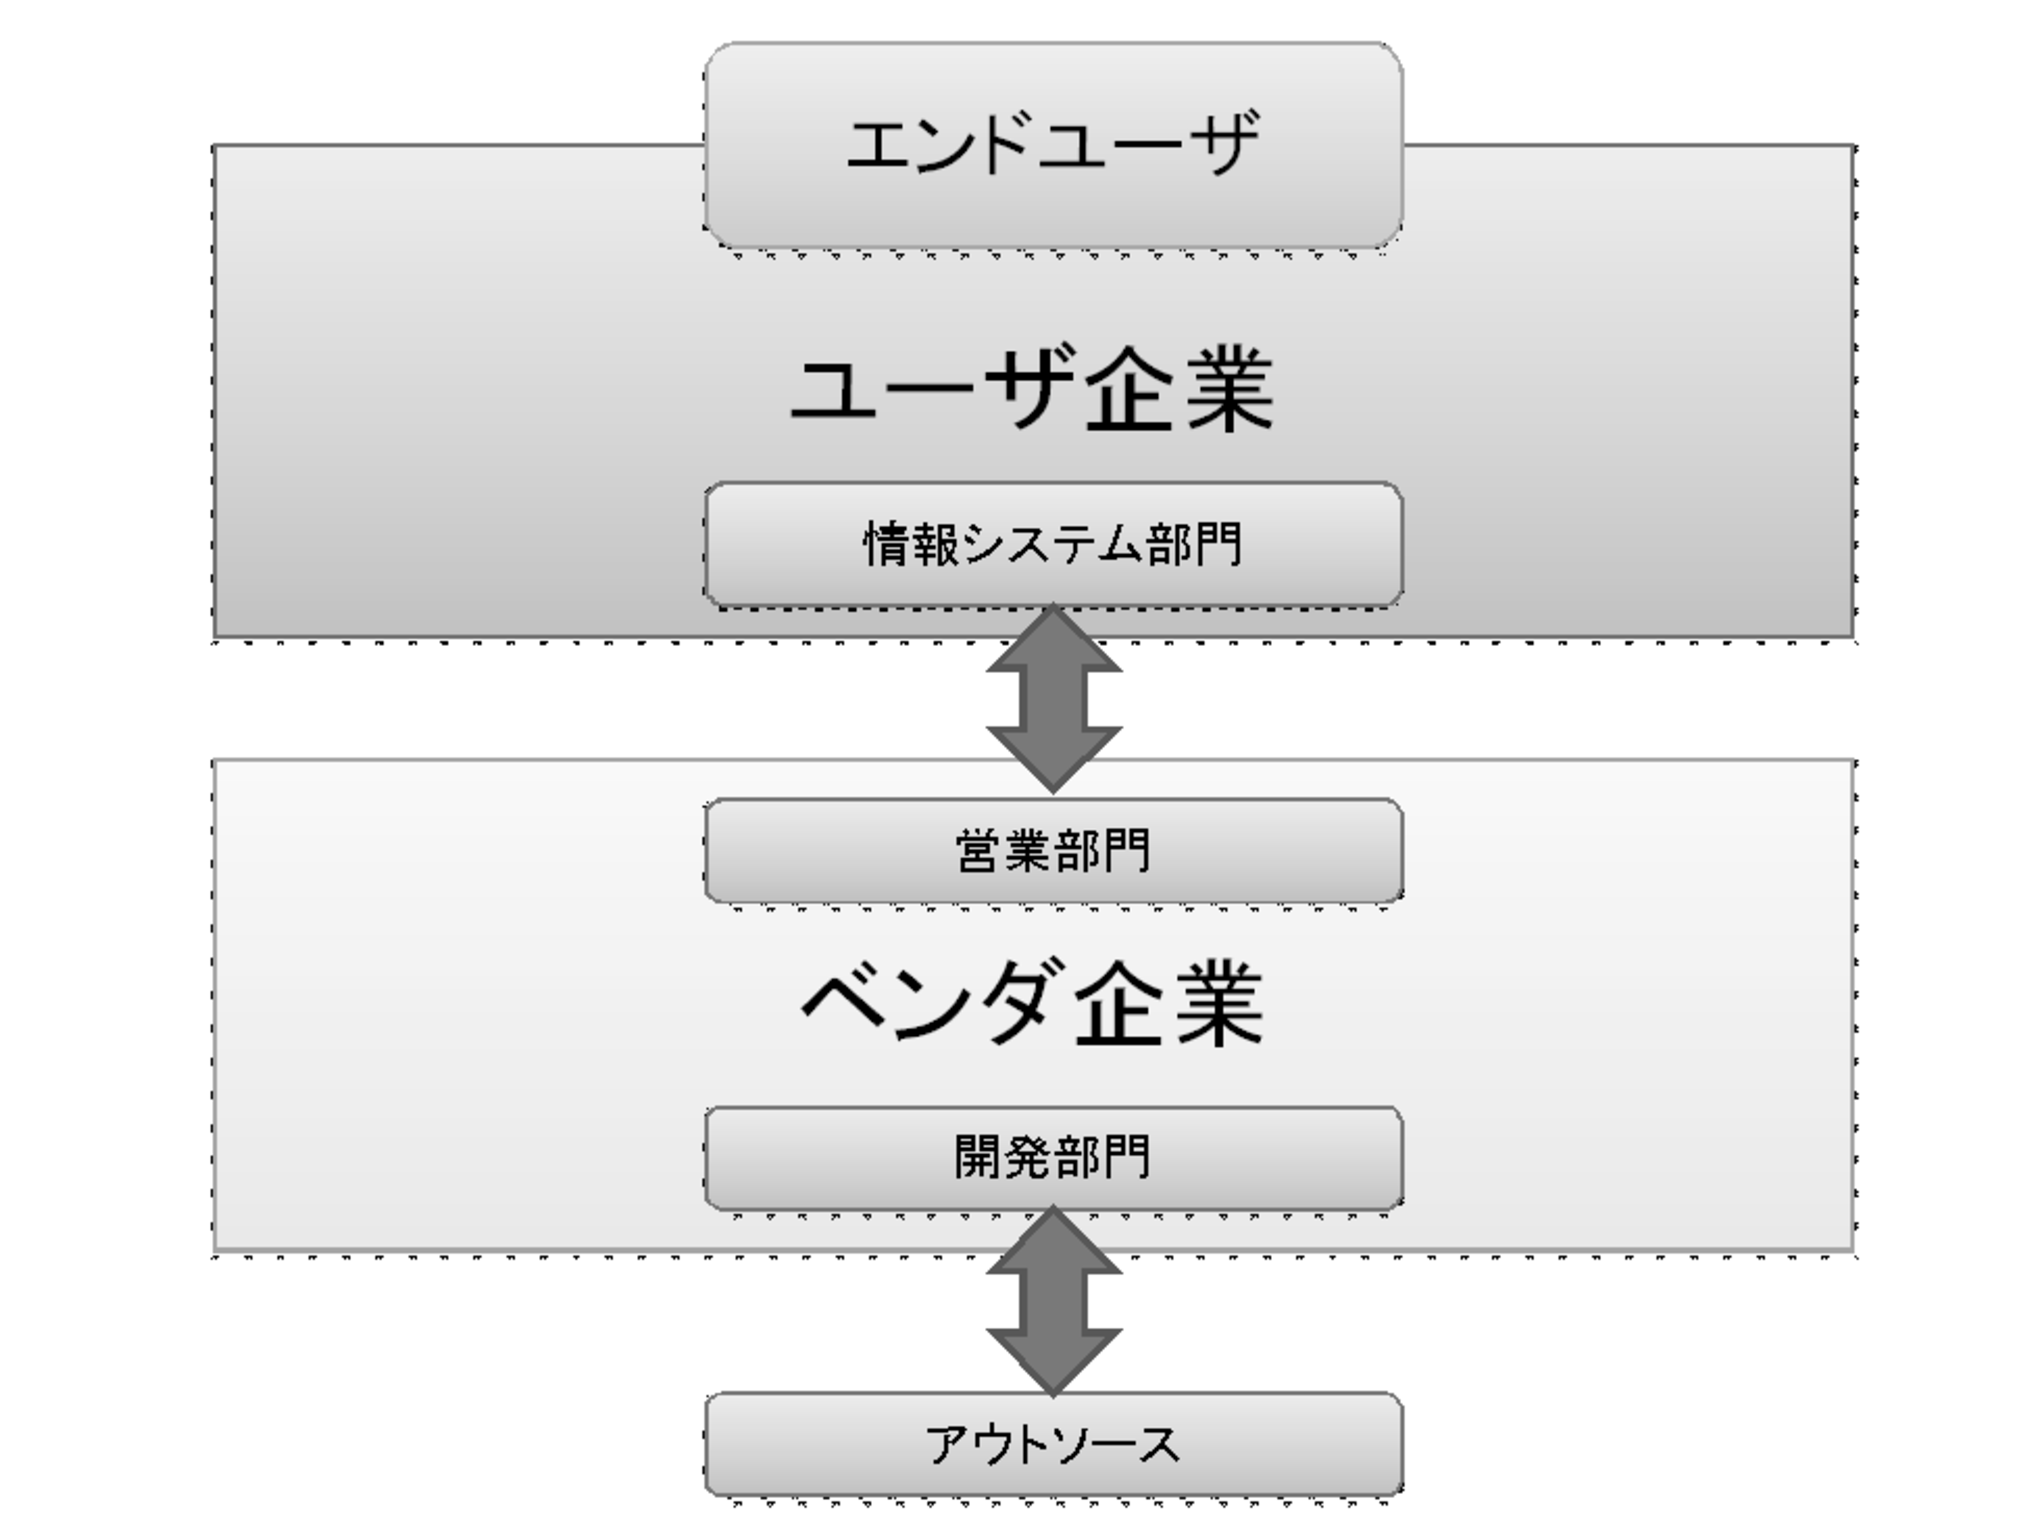
\includegraphics{figs/user_vendor_model.eps}}
\figcaption{ユーザ企業とベンダ企業の構造}
\label{fig:user_vendor_model}
\end{center}
	
\subsection{IT産業界の現状における構造的な問題}
    前項の目的を設定した背景には,{\bf 我が国におけるソフトウェア産業界の構造上の問題}がある.
	一般的なソフトウェア開発ビジネスにおいては    
    ITを提供するベンダ企業と,自社のサービスのためにITを利用するユーザ企業との間には
    明確な対立構造が存在する.
    このため,
    両者のコンフリクトをマネジメントすることがソフトウェア開発チームに求められ,
    {\bf コ・クリエイティブにソフトウェアを開発することが非常に難しい}.
    
    図\ref{fig:user_vendor_model}は,従来のソフトウェア開発における
    ユーザ企業とベンダ企業との関係構造を模式化したものである.
    本来,ベンダ企業にとっては実際にソフトウェアを利用するエンドユーザに有益なプロダクトを製造する
    ことが最大のミッションであるはずだ.
    ところが,エンドユーザとベンダ企業の開発部門やアウトソース先企業との間には
    図に示した通り,幾重にも壁が存在している.このため,
    {\bf エンドユーザが求めるソフトウェアを正しく製造することは構造的に困難}である.
    
    一番上に示した「エンドユーザ」とは,実際にソフトウェアを利用するユーザ(個人)である.エンドユーザは「ユーザ企業」に所属し,
    企業が提供するサービスを実現するために情報システムを利用する.近年は,B2C型でサービスを提供する企業が増えたことから,
    エンドユーザはユーザ企業の外部に存在し,Web等でユーザ企業が提供するサービスを利用する場合も見られる.
    
    このようなソフトウェア開発を行う場合,一般的にユーザ企業にある「情報システム部門」がシステム開発を主導することになる.
    情報システム部門は複数の「ベンダ企業」に対してRFP(Request For Proposal)を提示し,これを受けてベンダが作成した
    提案を精査し,ソフトウェア開発を発注するベンダ企業を選定する.この一連のプロセスはベンダ企業の「営業部門」が担当する.
    
    営業部門が契約を取り付けた後,ベンダ企業の「開発部門」が実際のソフトウェア開発プロジェクトを開始することになる.
    このとき,ベンダ企業内で必要なリソースが調達できない場合,ベンダ企業は社外の企業等に対して「アウトソース」を行う.
    いわゆる下請けの関係であり,近年は人件費の安い海外にアウトソースすることも多い.
    
    \subsection{IT産業の構造変化}

    翻って世界に目を向けると,以上述べてきた{\bf ユーザ企業とベンダ企業が対立する構造に依らない,
    新しいタイプのソフトウェア開発企業が登場}してきている.例えば,
    GoogleやFacebookなどの有力な企業は,自らの顧客であるユーザとインタネットを通じて
    直接的にコミュニケーションをしながら,
    自社のプロダクトをグローバルに提供することでビジネス的な成功を収めている.
    
    更に,App StoreやGoogle Playといったスマートフォン向けアプリの
    マーケットが登場しており,個人であっても直接ソフトウェアプロダクトをマーケットに投入することさえ容易になってきたことも,
    現在のソフトウェア産業における大きな構造変化である.
    
	\subsection{次世代のソフトウェア開発者チームの育成}

    ここまでの分析から,今後は{\bf 従来型の「ユーザ・ベンダ型モデル」は急速に存在感を失い,新しいタイプの企業が成長してくる}ものと予測する.
    本研究者はその際の中核概念が「コ・クリエイション」であると考える.
    
    すなわち,
    適時的にプロダクトをマーケットへ投入することで得られるマーケットからの``フィード・バック''や,
    将来的なマーケットの動向を予測して前もって製品に反映させる``フィード・フォワード''
    など,マーケットとの対話を通してプロダクトを生み出しうるソフトウェア企業が求められる.
    これは,マーケットとのコ・クリエーションのプロセスであり,
    その構造は図\ref{fig:CcSD}で示される.
    図\ref{fig:user_vendor_model}で示したモデルと比較すると,
    開発チームが直接マーケットとの対話を行う点で大きく異る.
    加えて,今後はグローバルなマーケットに対してのプロダクト開発も視野にいれておく必要があり,
    このような環境で迅速にソフトウェア開発ができる能力を備えた人材育成が望まれる.
    
\begin{center}
\scalebox{.21}{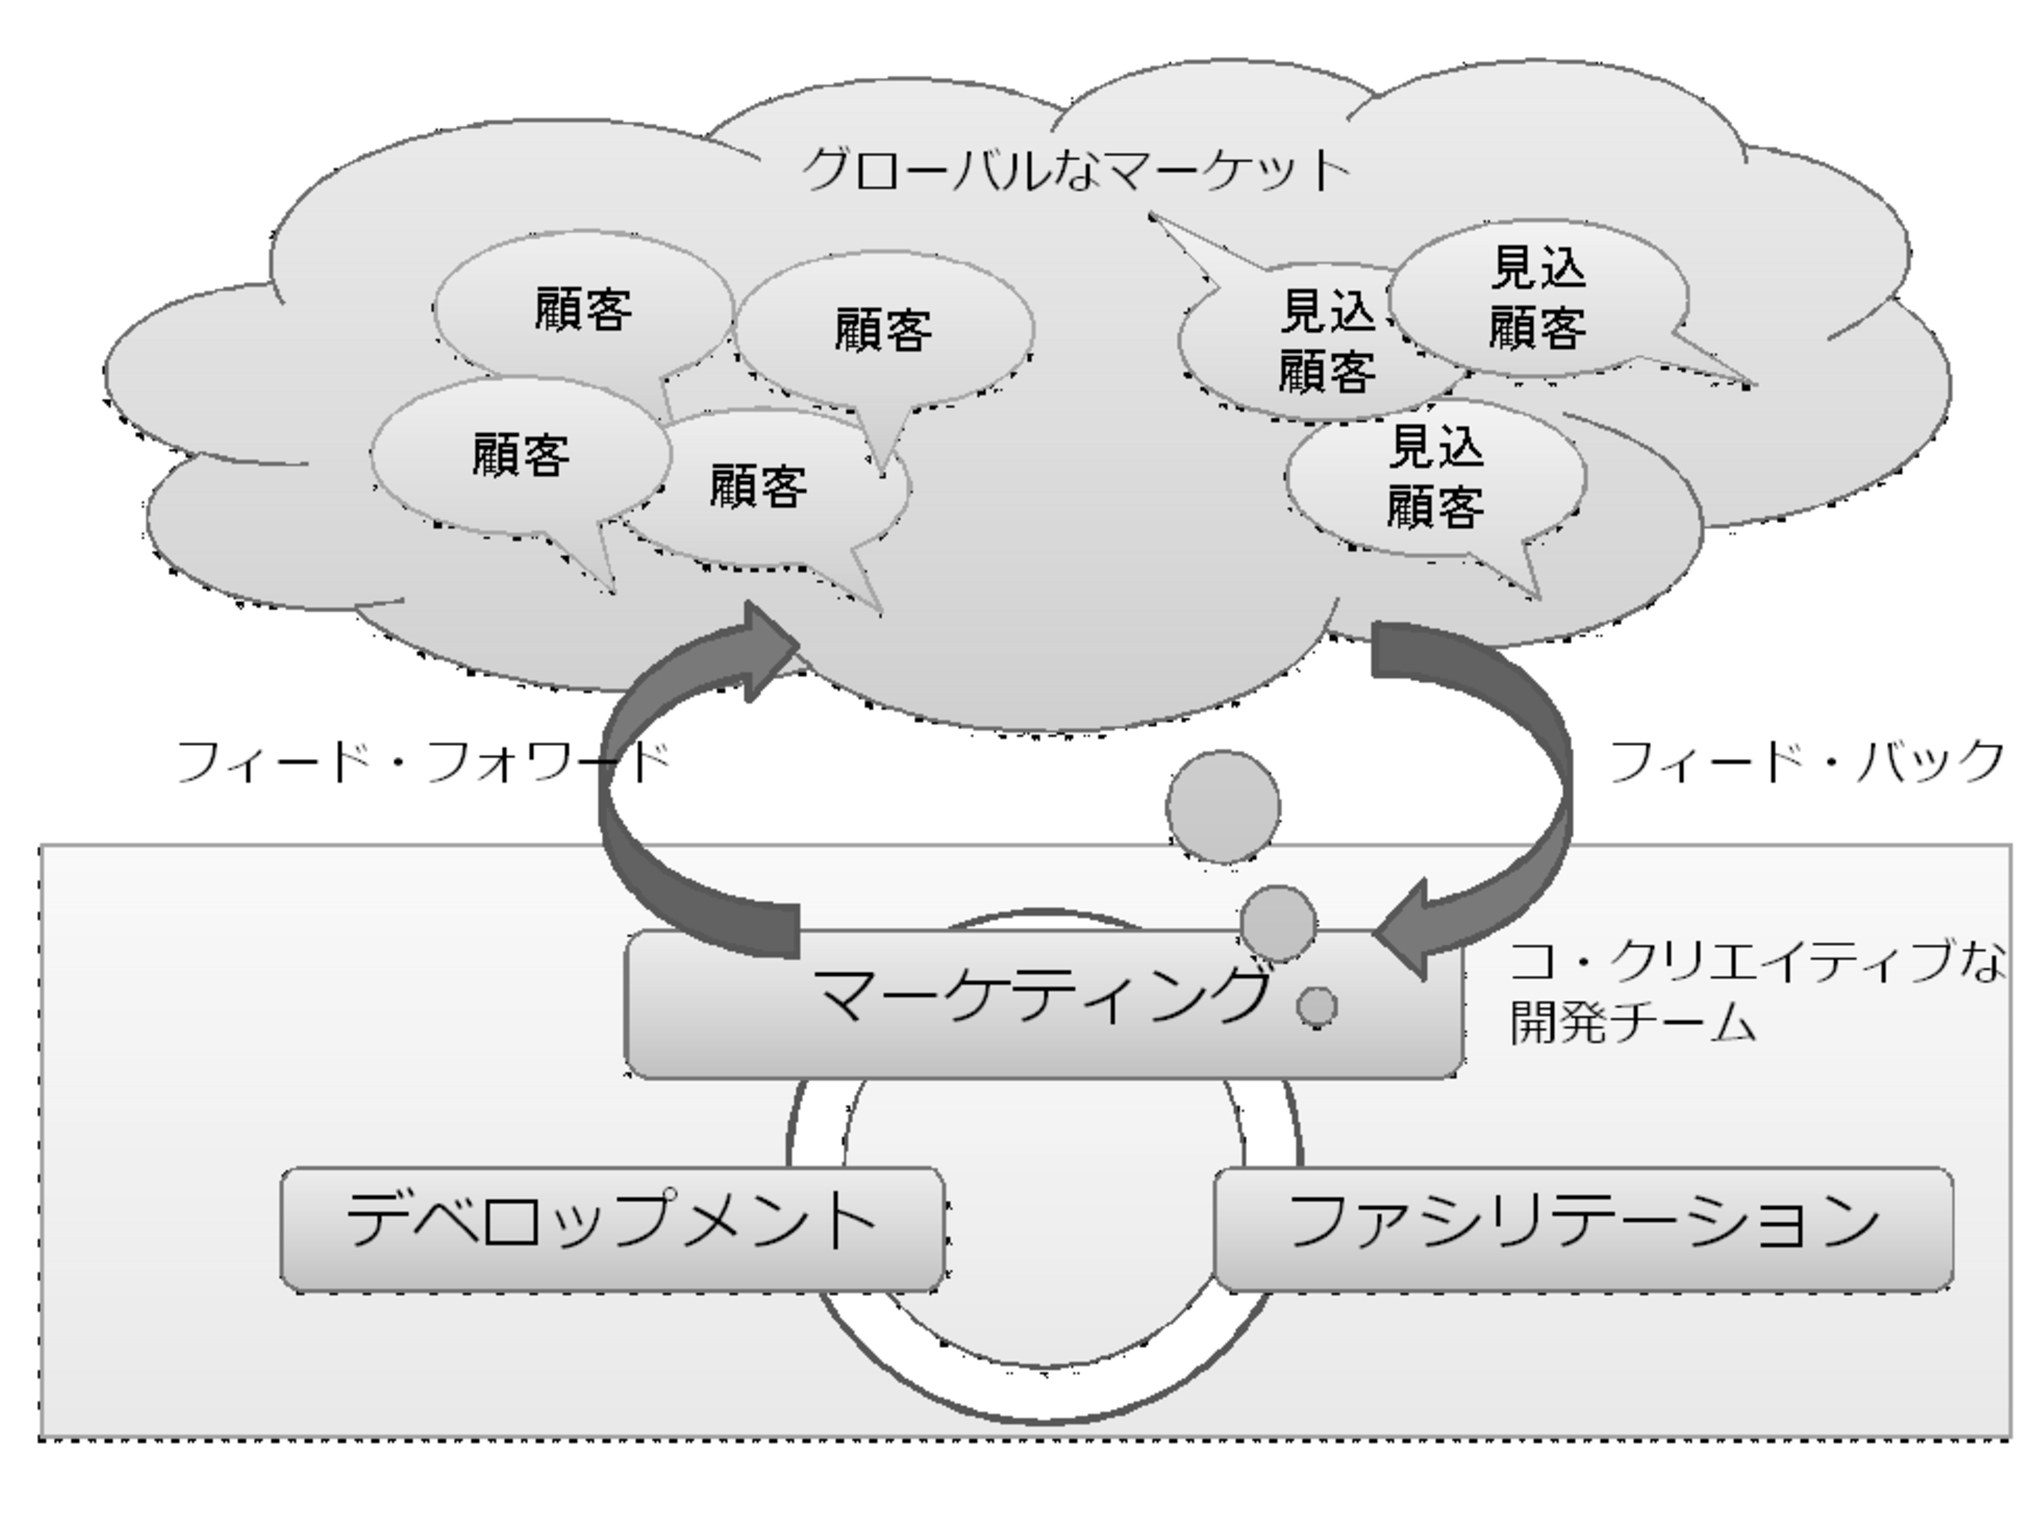
\includegraphics{figs/CcSD.eps}}
\figcaption{コ・クリエイティブなソフトウェア開発チームの振る舞い}
\label{fig:CcSD}
\end{center}
    
    そこで,本研究ではこの
    {\bf 「コ・クリエイティブ型ソフトウェア開発」に対応できる知識や技術を持った人材を育成するための
    新しい教材と教授法について研究開発}することを目的とする.
    近年,ソフトウェアの開発プロセスを教育するためのメソッドとして,
    PBLが効果を上げている\cite{pub:matsuzawa-2008}.
    ただし,既存のPBLではユーザ・ベンダ型の構造を前提とした上で,プロジェクトの中で
    それぞれのロールを体験することによる教育効果を狙ったものが多い.
    これでは産業構造の変化を踏まえた次世代の開発者を育成する内容として不十分である.
    特に,{\bf グローバルなマーケットとのコ・クリエイティブな対話}のプロセスや,そのベースとなる迅速なソフトウェア開発のための
    {\bf チームとしてのアジャイル性を獲得する方法の体得}を柱に再構成する必要があろう.
    
    以上の背景を踏まえ,次世代のソフトウェア開発者を育成するための
    {\bf 「コ・クリエイティブなソフトウェア開発者を育成するPBL型教育」の手法を確立}し,必要な教材やWebサービスとともにパッケージ化し,
    {\bf 様々な教育機関における教育に提供}できる成果を得ることを本研究の目的とする.

\section{研究の方法}
\subsection{ほげほげ}
	本研究では実施期間内においてアジャイル(迅速)に教材の開発と適用を繰り返し,より教育効果の高い
	PBL用電子教材を作成する.
	これには,迅速な電子教材開発のための「アジャイル教材製作スタジオ」を構築し,
	コンテンツとして用いる動画や音声を素早く製作できるように工夫する.
	製作した電子教材は,学生や教員がPBL実施時にオン・デマンドで参照できるようにし,
	学生の自発的な学びを支援する.

	初年度はScrum型の開発プロセスの教材を作成し,以降,コ・クリエイティブなソフトウェア開発のために
	必要な内容を拡充させる.成果物は本学および他大学でのPBLにおいて複数回利用し,改善を繰り返す.
	また,電子教材はクラウド型のサービスを用いて利用者に
	広く提供するものとする.
	
\begin{center}
\scalebox{.21}{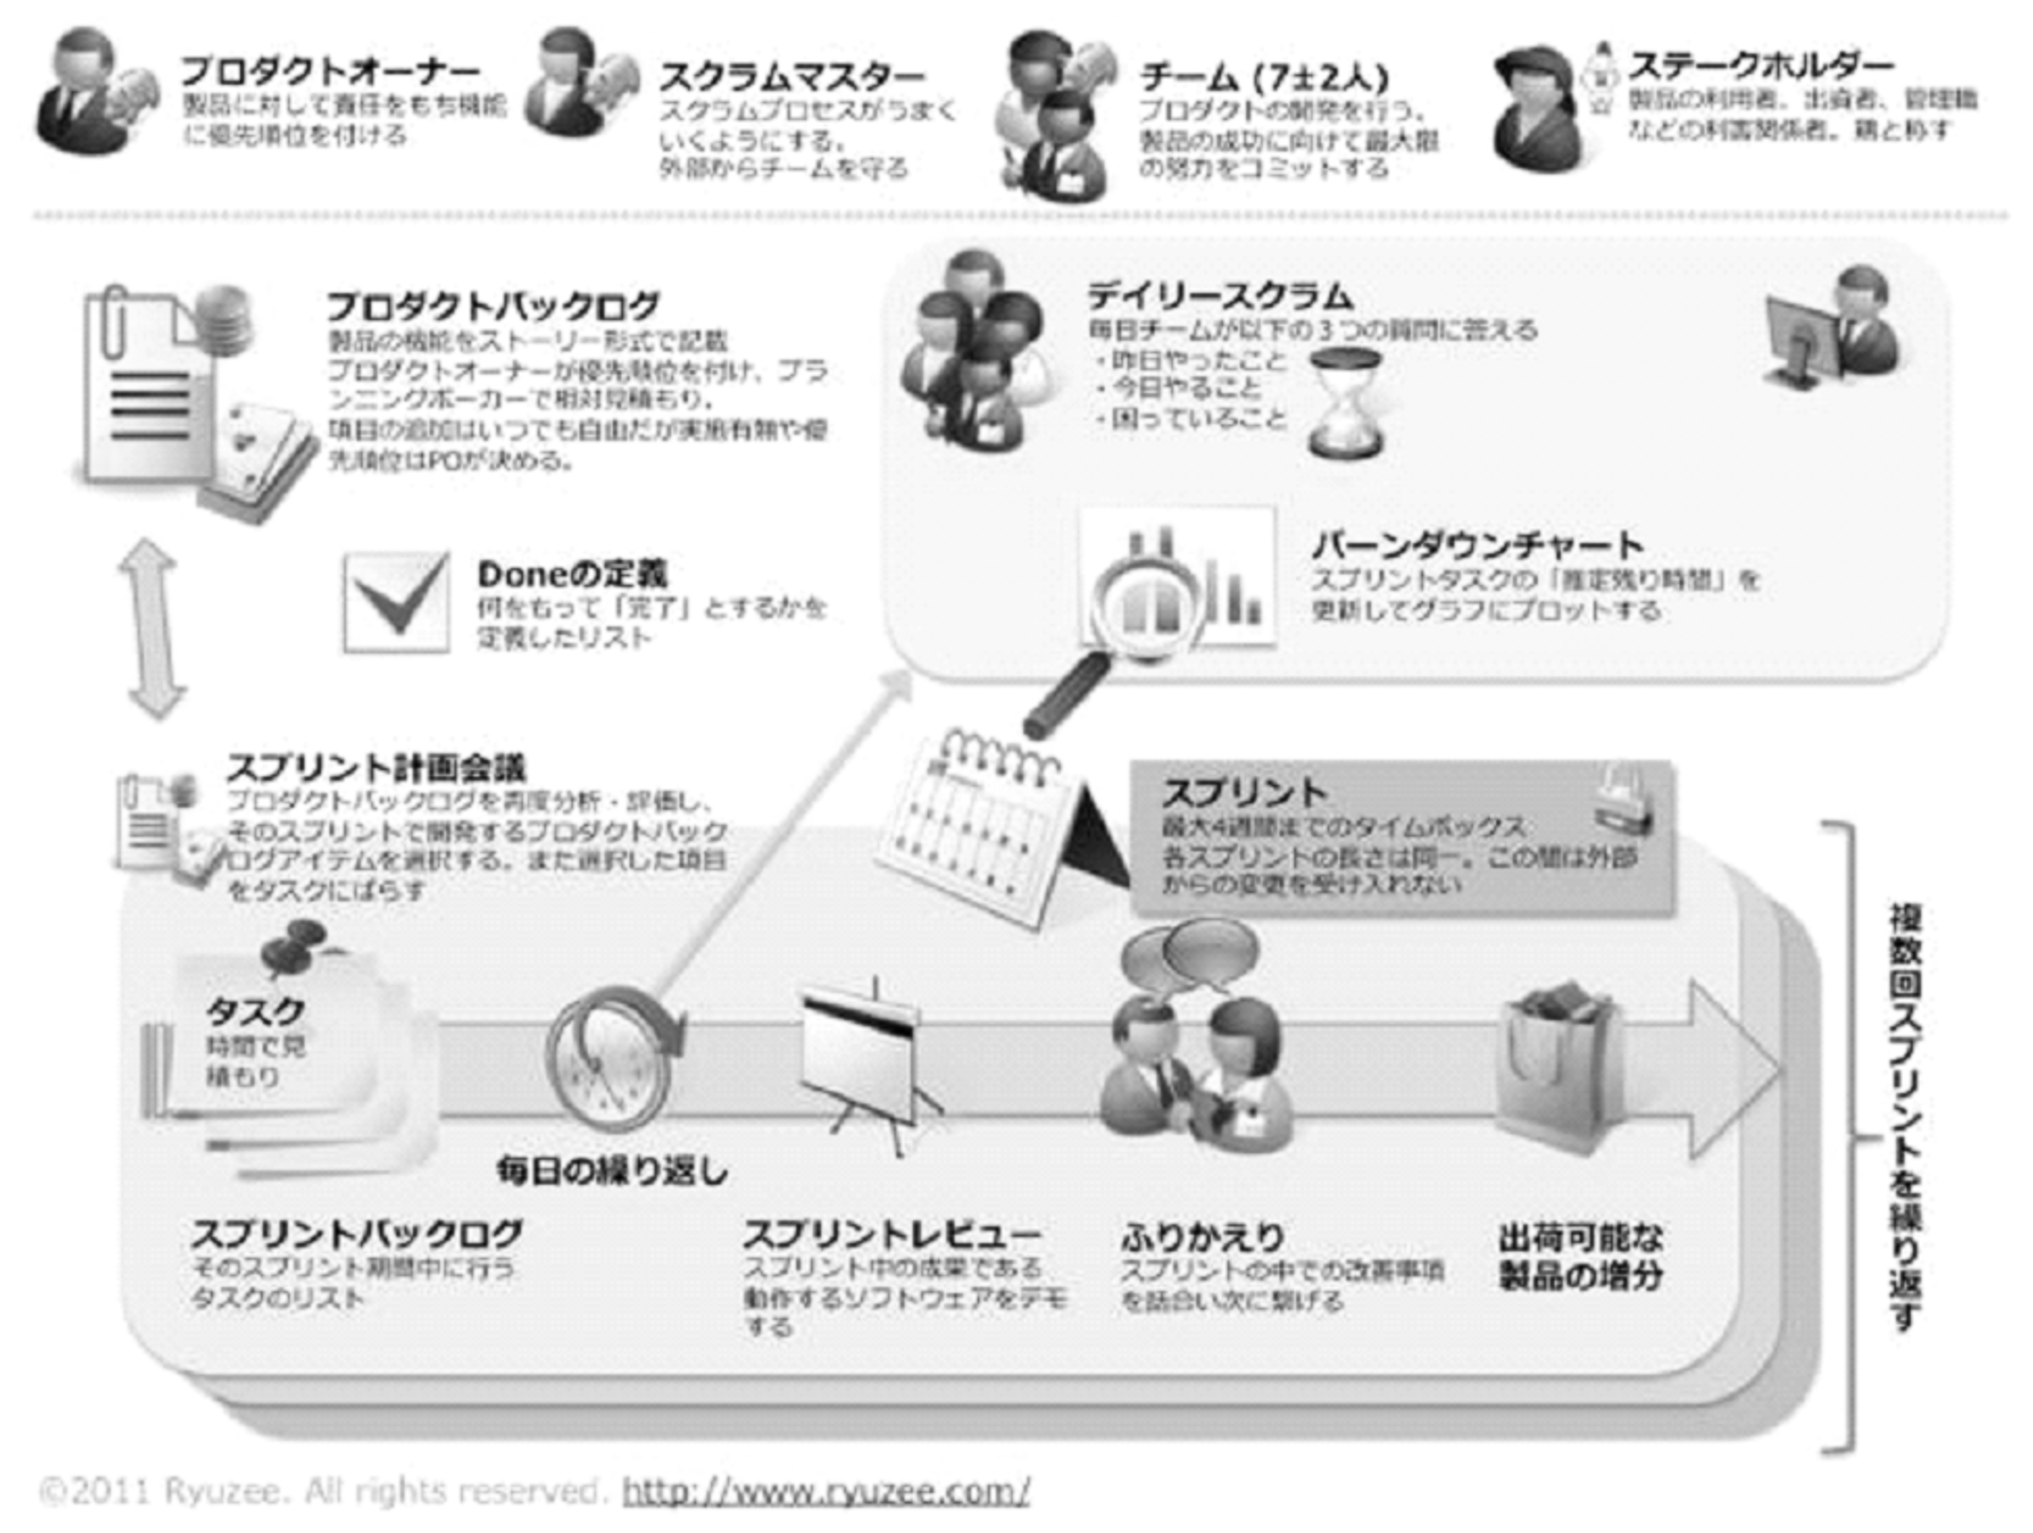
\includegraphics{figs/scrum.eps}}
\figcaption{Scrumの全体像(吉羽氏資料より)}
\label{fig:scrum}
\end{center}

\subsection{25年度の計画}
	
	アジャイルなソフトウェア開発プロセスとして近年注目されているScrumは,
	野中らが日本企業のベストプラクティスについて述べた文献\cite{nonaka}が起源だとされる.
	これをSutherlandらが1990年代半ばにソフトウェア開発プロセスとして定義した.
	{\bf Scrum は他のソフトウェア開発方式と比べて非常にシンプル}であり,
	その全体像は図\ref{fig:scrum}でほぼ網羅されている.このため
	学習すべき知識項目の数はさほど多くない.その反面,
	{\bf 実際にScrumをプロジェクトで実施できるようになるには相当の訓練が必要}である.

	このようなスキルの獲得のためにはScrum型でプロジェクトを行うPBLを実施することにより,高い教育効果が見込める.
	しかしながら,大学の教室で学生がScrumを学ぶことに適した既存の教材は見当たらない.また,指導する教員にとっても
	Scrumの概念を深く理解して学生を指導することは難しい.

	よって,研究初年度は{\bf Scrum型のプロセスを学習するためのPBL用教材を製作}
	することを目標とする.そのためのアプローチとして,Scrumを参考にしたアジャイルなプロセスを本研究の計画そのものにも取り入れ,
	{\bf アジャイルを学ぶ教材をアジャイルで製作する}という,ある種メタ的な手法をとる.
	研究自体をアジャイルで実施することの意義は,迅速に教材を作成し,授業を展開して効果を確かめ,さらなる改善を行うというプロセスを
	繰り返すことで,{\bf 教材の質を漸進的に向上}できることにある.
	
	{\bf Scrumはチームによる自己組織化や,作業プロセスの改善
	などを重視するのが特徴}である.
	これらは,実際にプロジェクトを行なってみて
	具体的な課題に直面してみないとその重要性に気づかないことが多い.
	そこで本研究で開発するScrum教育のための教材は,
	{\bf PBLを実施中の学生および教員がオンデマンドでアクセス}できる
	ようにする.
	これにより,学生がプロジェクトを実施中に具体的な課題に気づき,その解決を自主的に求めることを支援できるようになる.
	
	前述のとおり,
	本研究は研究自体もアジャイルで行うことため,迅速に教材を制作し,実際に教育の現場に教材を提供してフィードバックを得,
	必要な内容で漏れていることがあれば追加したり,わかりにくい箇所を改善させたりといった,反復型のプロセスにより
	内容を充実させていくことを基本的な計画とする.
	
	その最初のステップとしては,図\ref{fig:scrum}に基づき,Scrumの全体概要,
	役割分担(Scrum MasterやProduct Owner,Team Memberなど),
	成果物(プロダクトバックログ,スプリントバックログ,バーンダウンチャートなど),
	プロセス(スプリント計画会議,デイリースクラム,振り返りなど)に関する教材を用意しておく.
	加えて,Scrumで実際にソフトウェア開発を行うときに利用するクラウド型のツールについても解説する.

\begin{center}
\scalebox{.21}{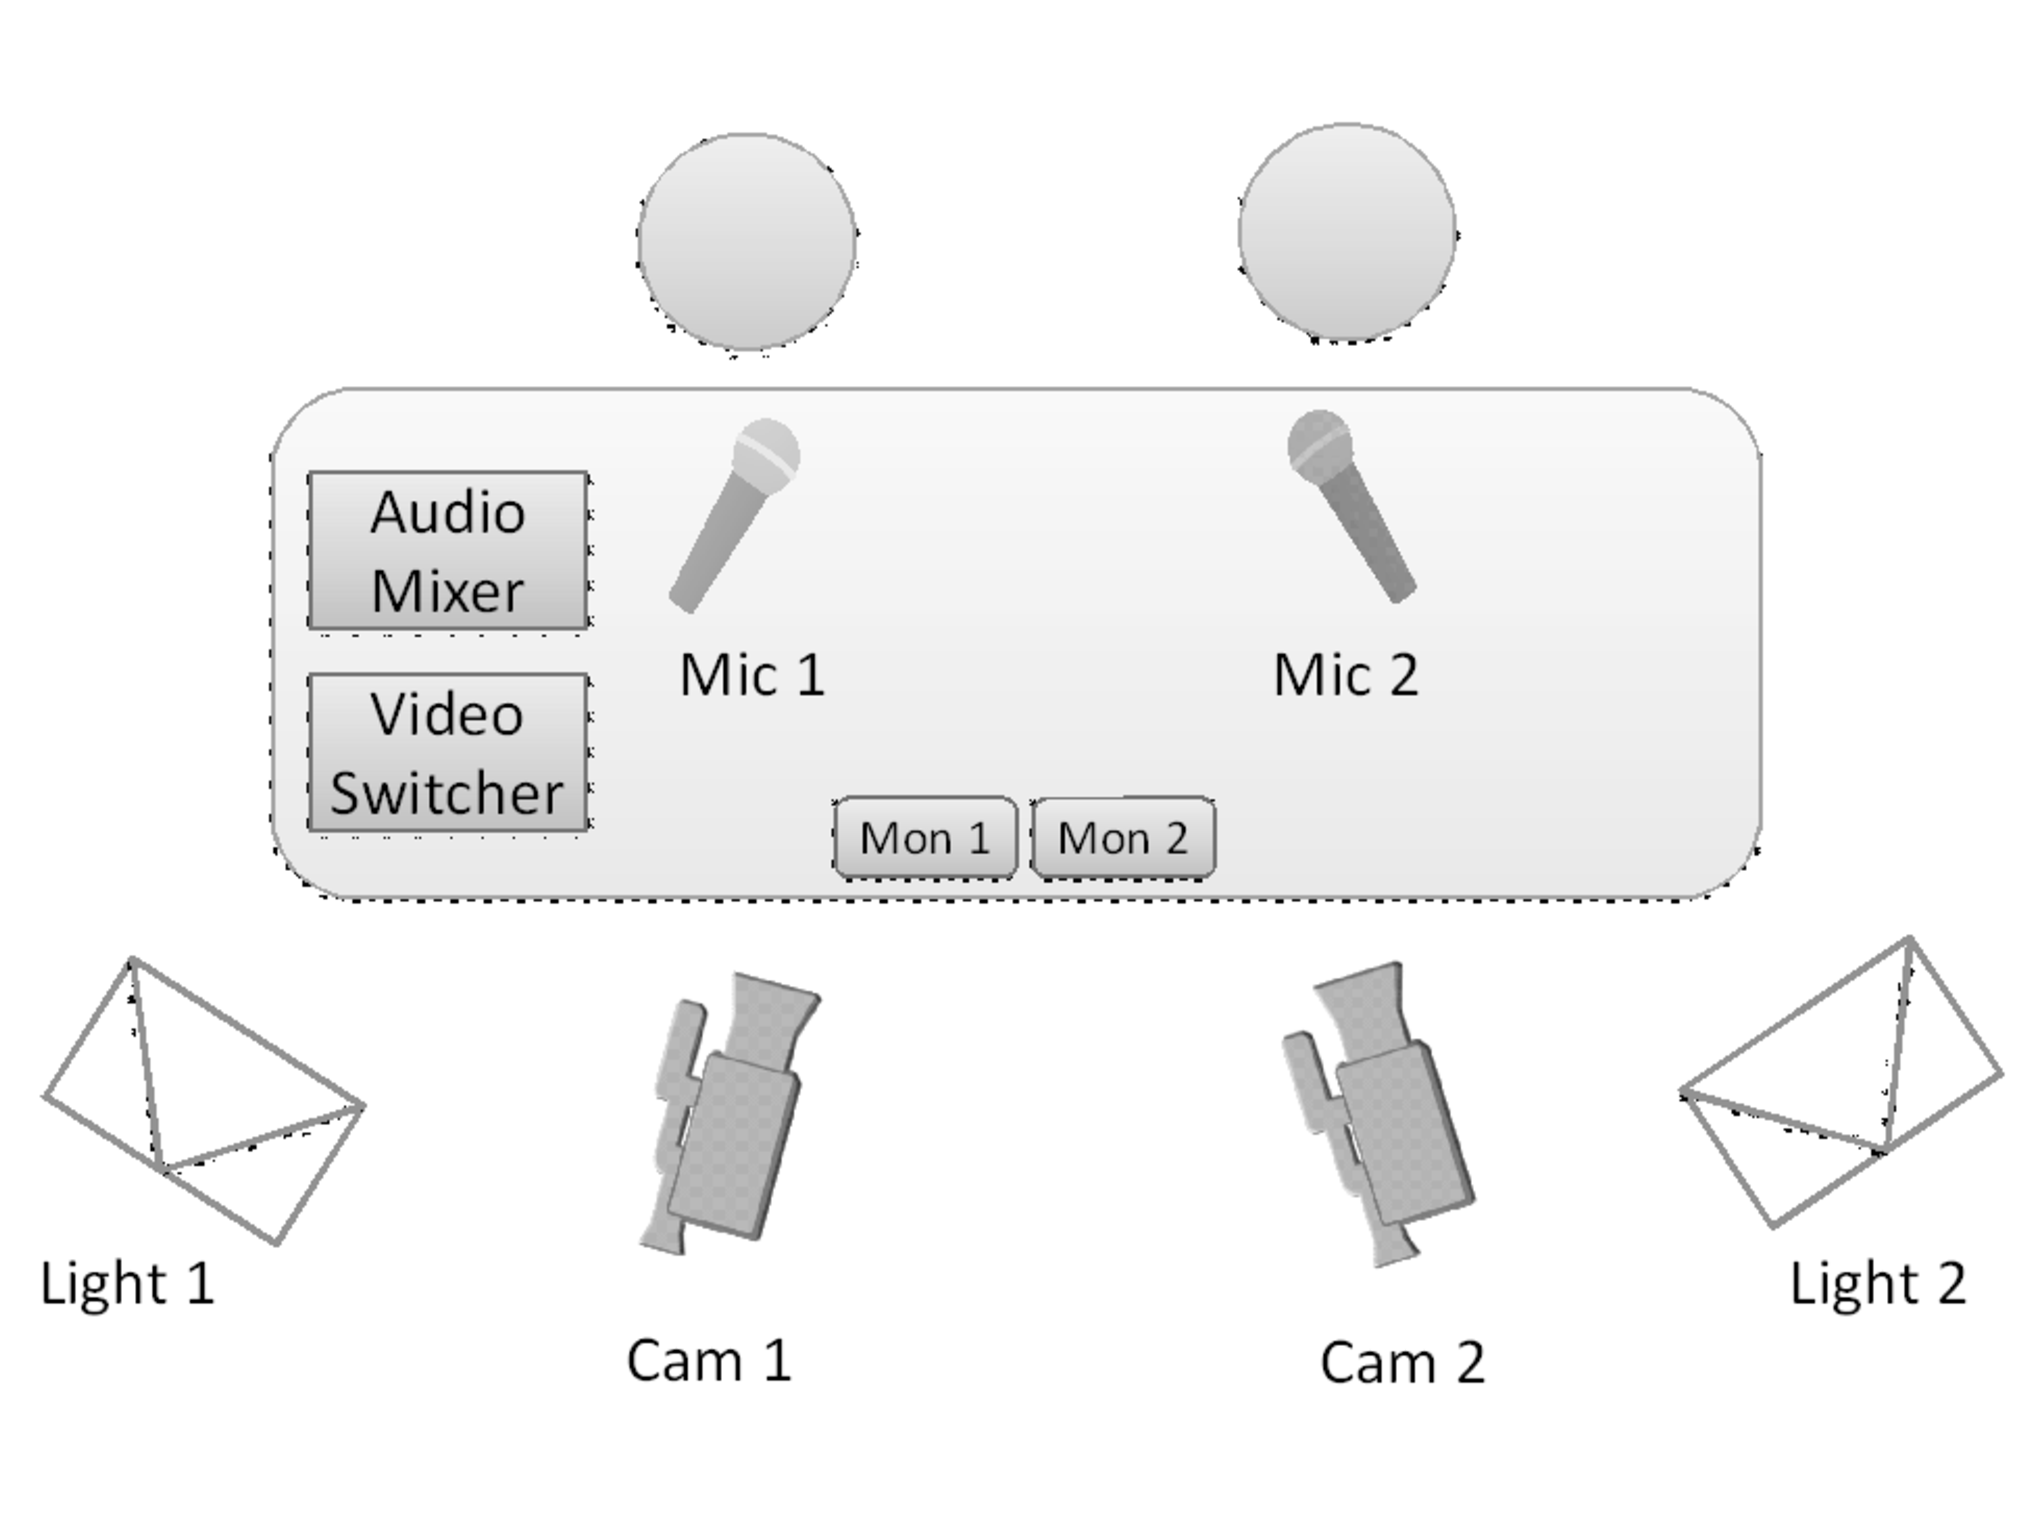
\includegraphics{figs/studio.eps}}
\figcaption{アジャイル教材制作スタジオ)}
\label{fig:studio}
\end{center}

	また,ゲーム感覚で取り組めるアンプラグドなワークショップを
	体験させるのもScrumの学習において効果的である.そこで,この教材では各種のワークショップ(紙飛行機作成,ボール渡し,
	Manager-Workerゲームなど多数)を紹介し,実施するための方法についても内容に含める.

	以上の研究計画を遂行する上での課題となるのは,音声や映像を伴う高クォリティの電子教材の製作に要する手間の低減である.
	そこで本研究では,
	業務でプロが使用するレベルの音響・映像機器(図\ref{fig:studio})と,
	様々な編集に必要となるコンピュータをセットにした{\bf 「アジャイル教材製作スタジオ」の構築}を研究テーマの1つとする.
	このスタジオにより迅速な電子教材製作を可能とすることを目指す.

	なお,本教材の研究開発全般において,Scrumコーチの認定資格を有する専門家に依頼し,内容等についてレビューして頂く.

	\begin{flushleft}
		■平成26年度以降の計画
	\end{flushleft}
	
	2年目からは,{\bf Scrumをベースとしたコ・クリエイティブ・ソフトウェア開発プロセスを学ぶための教材}
	を順次,追加する.

	クラウド技術などの発展により,開発したプロダクトをインターネット上にあるグローバルなマーケットに投入することが
	容易になってきている.学生が実施するPBLの成果物を現実のマーケットで公開し,
	その評価を得ることも難しくなくなった.
	
	そこで,
	{\bf PBLでの成果物を実際にマーケットに投入し,コ・クリエイティブにソフトウェアの製品価値を高める体験をするための教育コンテンツ}を追加する.
	加えて,各種のSocial Networkなどを利用して
	{\bf グローバルなコミュニケーションを通したコ・クリエイティブなソフトウェア開発}を行えるようにする教材開発にも取り組む予定である.

	本研究で得た知見は,本学におけるPBL型授業や,他大学(静岡大学・慶應大学等)の授業に随時導入し,その結果を積極的に発表する.
	発表する媒体としては,関連する学会等のほか,SNSやブログでも情報提供を行なっていく.
	これにより,{\bf 本研究における成果を広く社会に還元}するものとする.
	
	また,将来的には,作成した電子教材を各国語(英語,中国語・韓国語及びASEAN諸国の言語など)に翻訳し,
	海外の技術者と日本の学生とが共同で取り組むことのできるグローバルなPBLへと展開したい.
	
	\vspace{1cm}
	\begin{thebibliography}{99}
		\bibitem{wired} 顧客とのco-creationプラットフォーム-ベストプラクティ, \\
                        http://wired.jp/2011/09/29/,  2012-10-24参照
        \bibitem{oss} クリス・ディボナ他, オープンソースソフトウェア―彼らはいかにしてビジネススタンダードになったのか,
        				オライリー・ジャパン, 1999-07
		\bibitem{nonaka} H.~Takeuchi, I.~Nonaka: The New New Product Development Game, Harvard Business Review January-February, 1986
		% \bibitem{lean-startup} エリック・リース: リーン・スタートアップ ―ムダのない起業プロセスでイノベーションを生みだす, 日経BP社, 2012
		\bibitem{pub:chubachi-ipbl-2012} \me, 小山裕司: AIITにおけるプロジェクト型学修(PBL)のためのBacklogシステムの導入, 情報処理学会 第19回IOT・第39回EVA合同研究発表会, 島根県松江市, 2012-09-27.(査読無) 
% 		\bibitem \me, 小山 裕司, 石島 辰太郎: 産業技術大学院大学のICT環境の運用と課題, 研究報告インターネットと運用技術(IOT), 一般社団法人情報処理学会, Vol.2012-IOT-16, No.11, pp.1-4, 2012-03-08.(査読無)
% 		\bibitem 野口 靖浩, \underline{松澤 芳昭}, 森 孝夫,島 聰司,塩見 彰睦:合宿とPBLによる組込みシステムアーキテクト養成プログラムの設計と評価,日本教育工学会論文誌,Vol.36, No.1, pp.21-33, 2012. (査読有)
% 		\bibitem 野口 靖浩, \underline{松澤 芳昭}, 島 聰司, 塩見 彰睦: 組込み人材育成研修後の上司による「行動変容」評価の実践とSCATによる分析, 工学教育, Vol.60, No.3, pp.86-91, 2012.05. (査読有)
		\bibitem{pub:chubachi-ipbl-2011}\me, 小山 裕司: PBLを支援するコラボレーティブツールに関する考察, 産業技術大学院大学紀要, No.5,pp.100-108, 2011 (査読有)
% 		\bibitem 小山 裕司, \me, 土屋 陽介: ソーシャルメディアを活用したコネクション構築支援, 情報処理学会研究報告. コンピュータと教育研究会報告, 一般社団法人情報処理学会, Vol.2011, No.3, pp.1-6, 2011-12-10.(査読無)
% 		\bibitem 土屋 陽介, 小山 裕司, \me: 授業配信システムの設計と開発, 情報処理学会研究報告. コンピュータと教育研究会報告, 一般社団法人情報処理学会, Vol.2011, No.2, pp. 1-7, 2011-12-10.(査読無)
		\bibitem{pub:kizaki-global-2011b} 木崎 悟, 成田 亮, 丸山 英通, 土屋 陽介, 成田 雅彦, \me: 国際PBLにおける的確な仕様の伝達とチケット駆動による開発作業の効率化, ソフトウェアエンジニアリングシンポジウム2011, 東京女子大学, 2011-09.(査読有)
		\bibitem{pub:kizaki-global-2011c} 木崎 悟, 丸山 英通, 土屋 陽介, \me: ソフトウェア開発PBLへのチケット駆動開発の適用による共同作業の改善, プロジェクトマネジメント学会 2011年度秋季研究発表大会, 産業技術大学院大学, 2011-09.(査読無)
		\bibitem{pub:kizaki-global-2011a} 木崎 悟, 成田 亮, 丸山 英通, \me: グローバルなソフトウェア開発におけるマネジメント手法, 情報処理学会 第172回ソフトウェア工学研究会, 早稲田大学, 2011-05-17.(査読無)
		\bibitem{pub:chubachi-global-2010} \me, 成田 雅彦, 戸沢 義夫: 加藤由花, 戸沢義夫: ベトナム国家大学とのグローバル PBL から得た知見, 産業技術大学院大学紀要, pp.1-4, 2010. (査読有)
% 		\bibitem \me: 遠隔会議システムを用いた国際PBLから得た知見, 日本e-Learning学会学術講演会論文誌, 東京都千代田区, 2010-11-14.(査読無)
% 		\bibitem \meen, Y.~Kato, Y.~Tozawa: Web-based groupware supporting PBL effectively, 1st Asia-Pacific Joint PBL Conference 2010, 2010-10-24(査読有)
		\bibitem{pub:nishino-2010} R.~Nishino, M.~Kojima, O.~Oka, T.~Okino, T.~Sugita, Y.~Tsuchiya, H.~Koyama, Y.~Tozawa, \meen: Experience Gained through International PBL in Software Development, 1st Asia-Pacific Joint PBL Conference 2010, 2010-10-23(査読有)
% 		\bibitem \me, 小山 裕司, 石島 辰太郎: ICTを基盤とした高度専門職教育, 情報教育シンポジウム論文集, 情報処理学会, 情報処理学会シンポジウムシリーズ IPSJ Symposium Series Vol.2010, No.6, pp.133-138, 群馬県渋川市, 2010-08-19.(査読無
% 		\bibitem Y.~Matsuzawa, Y.~Noguchi, T.~Mori, S.~Shima, A.~Shiomi: ESAD: An Intensive Retreat Program for Embedded System Architect Developing, 17th APSEC, pp.90-97, 2010.(査読有)
% 		\bibitem Y.~Matsuzawa, J.~Oshima, R.~Oshima, Y.~Nihara, S.~Sakai: KBDeX: A Platform for Exploring Discourse in Collaborative Learning, Collaborative Innovation Networks(COINs) 2010. (Web出版) (査読有)
		\bibitem{pub:chubachi-ipbl-2009b} \me, 加藤由花, 戸沢義夫: PBL用情報インフラストラクチャの構築と運用, 産業技術大学院大学紀要, pp.109-116, 2009 (査読有)
		\bibitem{pub:tozawa-pbl-2009} Y.~Tozawa, Y.~Kato, \meen: Efforts to ensure the quality of PBL education in the graduate school of Information Technology, Proceedings of the 2nd International Research Symposium on PBL, 3-4 December 2009, Melbourne, Australia, pp.1-9(査読有)
%		\bibitem \me: 要求分析モデリング支援システムの開発~SBVAエディタ~, 要求工学ワーキンググループ ワークショップ, 情報処理学会, 天橋立, 2009-10-22
		\bibitem{pub:tozawa-global-2009} 戸沢 義夫, 成田 雅彦, \me, 土屋 陽介: Global PBL Feasibility Studyの実践と得られた知見, 情報処理学会 情報教育シンポジウム論文集, pp.167-174,2009-08-20.(査読無)
		\bibitem{pub:ohrui-global-2009} 大類 優子,成田 雅彦,\me,土屋 陽介,戸沢 義夫: Global PBL Feasibility Studyの実践検証, 情報科学技術フォーラム講演論文集, FIT(電子情報通信学会・情報処理学会)推進委員会, 2009-08-20, Vol.8, No.4, pp. 515-516
		\bibitem{pub:chubachi-ipbl-2009a} \me, 土屋 陽介, 長尾 雄行, 加藤 由花, 酒森 潔, 戸沢 義夫: グループウェア導入によるPBLの見える化, 日本e-Learning学会論文誌, Vol.9, pp.129-135, 2009-05.(査読有)
% 		\bibitem \me: 要求記述演習によるロジカルシンキング教育の評価, 要求工学ワーキンググループ ワークショップ, 情報処理学会, 銚子, 2009-05-29
%       \bibitem \me: 要求分析者育成のためのコミュニケーション能力教育, ウィンターワークショップ2009・イン・宮崎論文集, 情報処理学会, Vol.2009, No.3, pp.45-46, 宮崎, 2009-01-23
% 		\bibitem \me: 要求工学セッションの紹介~WW2010~, ウィンターワークショップ2010イン・倉敷論文集,情報処理学会,情報処理学会シンポジウムシリーズ IPSJ Symposium Series Vol.2010,No.3, pp.31-32, 2010-01-21
% 		\bibitem Y.~Matsuzawa, A.~Shiomi, T.~Haraikawa, S.~Sakai: Two Challenges to Promote EVM on PBL in Software Engineering Education, 2nd International Research Symposium on PBL (IRSPBL'09), pp.1-10, 2009.(査読有)
% 		\bibitem 松澤 芳昭,大岩 元: 情報系学生を対象としたオブジェクト指向までのプログラミング入門教育の実践と課題, 情報教育シンポジウム(SSS2009),pp199-206, 2009.(査読有)
% 		\bibitem 長尾 雄行, 土屋 陽介, 森本 祥一, \me: JavaScriptと非同期HTTPリクエストによる共同作業支援ミドルウェアの構築, 産業技術大学院大学紀要, Vol.2, pp.165-174, 2008(査読有)
% 		\bibitem 森本 祥一, \me: シナリオの図解化による業務フロー分析, 産業技術大学院大学紀要, Vol.2, pp.193-208, 2008(査読有)
% 		\bibitem \me, 土屋 陽介, 長尾 雄行, 加藤 由花, 酒森 潔, 戸沢 義夫, PBLを見える化する協調作業支援環境の構築, 日本e-Learning学会2008年秋季学術講演会論文集, pp.72-79, 京都, 2008-11.(査読無) ※優秀賞受賞
% 		\bibitem \me, システム開発における仮説検証型の要求分析プロセス, 要求工学ワーキンググループ ワークショップ, 情報処理学会, 雲仙, 2008-10-23
% 		\bibitem 長尾 雄行, 土屋 陽介, 森本 祥一, \me: JavaScriptと非同期HTTPリクエストによる共同作業支援ミドウェアの構築, 情報処理学会論文誌:プログラミング, Vol.1, No. 1, pp.63-64, 2008-06
% 		\bibitem \me, 専門職大学院におけるモデリング教育とSBVA法, 要求工学ワーキンググループ ワークショップ, 情報処理学会, 奄美大島, 2008-05-15
% 		\bibitem 橋山 牧人,中鉢 欣秀, 大岩 元: 携帯ゲームアプリケーション開発を支援するオブジェクト指向を用いたフレームワークの開発, 情報処理学会第71会全国大会, pp.4-733-734,草津(滋賀), 2009年3月 (NII)
% 		\bibitem 杉浦 学,\underline{松澤 芳昭},岡田 健,大岩 元: アルゴリズム構築能力育成の導入教育:実作業による概念理解に基づくアルゴリズム構築体験とその効果,情報処理学会論文誌,Vol.49,No.10,pp.3409-3427, 2008(査読有)
% 		\bibitem 荒木 恵, \underline{松澤 芳昭},杉浦 学,大岩 元: プログラミング教育への導入のための情報システム概念に基づくアンプラグドワークショップ,情報教育シンポジウム(SSS2006),pp.163-170, 2008(査読有)
		\bibitem{pub:matsuzawa-2008} 松澤 芳昭,杉浦 学,大岩 元: 産学協同のPBLにおける顧客と開発者の協創環境の構築と人材育成効果, 情報処理学会論文誌,  Vol.49, No.2, pp.944-957, 2008(査読有)
	\end{thebibliography}

\newpage % 消さないで

\end{multicols}
\end{document}


\section{標題等について}
\subsection{原稿}
原稿は,日本語もしくは英語による完全版下(camera ready)原稿とする.製版後の校正は原則として不可能であるため,誤字や脱字がないよう,特に念を入れて仕上げる.刷り上がりは,6頁以上が望ましい.

\subsection{標題}
標題は和文ならびに英文とする.英文原稿の場合は,和文表題を記述するところに英文標題を記述し,通常の英文標題のところは削除すること.

\subsection{著者名・所属}
著者名も英文による原稿の場合は,通常の和文著者名のところに英文で記述し,英文著者名のところは削除すること.所属も英文で記述すること.

\subsection{アブストラクト・キーワード}
和文ではなく英文で記述すること.アブストラクトは100語程度とし,キーワードは5つ程度とする.

\subsection{標題等の割付}
別紙産技大紀要カメラレディ用見本に従って,[和文標題,和文著者名,英文標
題,英文著者名,英文アブストラクト,英文キーワード,所属]の割付を行う.

\section{本文について}

\subsection{余白}
天地左右余白(マージン)・段間余白(コラムスペース)も産技大紀要カメラレディ用見本に従う.

\subsection{見出し}
原稿には,大見出し,中見出しなどを設け,それらを明瞭に区分する.さらに細分を要するときは,著者の分類に委ねる.

\subsection{句読点}
句読点には,全角ピリオド(.),全角コンマ(,)を用いること.

Lorem ipsum dolor sit amet, consectetur adipiscing elit. Aenean sed
nulla nisi. Pellentesque habitant morbi tristique senectus et netus et malesuada
fames ac turpis egestas. Aliquam erat volutpat. Sed tristique ipsum eu nisl
viverra a accumsan elit ultricies. Fusce porta eros a lectus scelerisque vitae
eleifend odio interdum. Pellentesque habitant morbi tristique senectus et netus
et malesuada fames ac turpis egestas. Aliquam erat volutpat.

\section{図・表について}
\subsection{キャプション}
図・表には,図1,図2,表1,表2 のように論文全体で通し番号をつけること.
表のキャプションは表の上に,図のキャプションは図の下につけること.図・表
ともに配置は中央揃えにすること.

英文の場合には,Fig. 1,Fig. 2,Table 1,
Table 2のように,番号をつけること.通し番号,標題は本文と同じ書体を使用
すること.

multicols を用いたため figure 環境,table 環境は使えない.
通常の caption が使えないため.代わりに figcaption,tblcaption を用いて
図と表の caption をつけること.以下に例を示す.

%%%%%%%%%%%%%%%%%%%%%%%%%%%%%%%%%%%%%%%%%%%%%%%%%%%%%
%%%                   Fig                       %%%
%%%%%%%%%%%%%%%%%%%%%%%%%%%%%%%%%%%%%%%%%%%%%%%%%%%%%
\begin{center}
\scalebox{.21}{
\includegraphics{aiit_logo.eps}}
\figcaption{図のキャプション}
\label{fig:VFS}
\end{center}
%%%%%%%%%%%%%%%%%%%%%%%%%%%%%%%%%%%%%%%%%%%%%%%%%%%%%
%%%                    Table                      %%%
%%%%%%%%%%%%%%%%%%%%%%%%%%%%%%%%%%%%%%%%%%%%%%%%%%%%%
\tblcaption{表のキャプション}
\label{tab:cost2}
\begin{center}
\begin{tabular}{|c|c|c|} \hline
A & B & C \\ \hline
$A_{1}$ & $B_{1}$ & $C_{1}$ \\ \hline
$A_{2}$ & $B_{2}$ & $C_{2}$ \\ \hline
$A_{3}$ & $B_{3}$ & $C_{3}$ \\ \hline
$A_{4}$ & $B_{4}$ & $C_{4}$ \\ \hline
\end{tabular}
\end{center}

\subsection{図の中の文字等}
 図・表は,印刷に十分耐えうるものでなければならない.刷り上がり時の文字が小さすぎないよう十二分に配慮し,線の太さにも注意する.

\subsection{色刷り}
図・表に色刷りを必要とする場合は,別途連絡すること.ただし,製本上の都合で色刷り頁を設けることができない場合もありうる.

\section{参考文献について}
参考文献は,通し番号とし,本文中では,当該事項または人名などの参考とする
後に,\cite{TRA96HuHaCo},\cite{SICE02Yo}--\cite{Asa02Ar}
のように記す.文章の末尾に記す必要がある場合には,句読点の前に記す.参考文献は,原則として,雑誌の場合は,著者,標題,雑誌名,巻,号,頁,年の順に記す.また,著書の場合は,著者,書名,発行所,発行年の順に記す.参考文献例を本文の最後に挙げるので参考されたい.

\section{おわりに}
本稿では産業技術大学院大学紀要のフォーマットについて記した.

Lorem ipsum dolor sit amet, consectetur adipiscing elit. Aenean sed
nulla nisi. Pellentesque habitant morbi tristique senectus et netus et malesuada
fames ac turpis egestas. Aliquam erat volutpat. Sed tristique ipsum eu nisl
viverra a accumsan elit ultricies. Fusce porta eros a lectus scelerisque vitae
eleifend odio interdum. Pellentesque habitant morbi tristique senectus et netus
et malesuada fames ac turpis egestas. Aliquam erat volutpat.

Lorem ipsum dolor sit amet, consectetur adipiscing elit. Aenean sed
nulla nisi. Pellentesque habitant morbi tristique senectus et netus et malesuada
fames ac turpis egestas. Aliquam erat volutpat. Sed tristique ipsum eu nisl
viverra a accumsan elit ultricies. Fusce porta eros a lectus scelerisque vitae
eleifend odio interdum. Pellentesque habitant morbi tristique senectus et netus
et malesuada fames ac turpis egestas. Aliquam erat volutpat.

Lorem ipsum dolor sit amet, consectetur adipiscing elit. Aenean sed
nulla nisi. Pellentesque habitant morbi tristique senectus et netus et malesuada
fames ac turpis egestas. Aliquam erat volutpat. Sed tristique ipsum eu nisl
viverra a accumsan elit ultricies. Fusce porta eros a lectus scelerisque vitae
eleifend odio interdum. Pellentesque habitant morbi tristique senectus et netus
et malesuada fames ac turpis egestas. Aliquam erat volutpat.

Lorem ipsum dolor sit amet, consectetur adipiscing elit. Aenean sed
nulla nisi. Pellentesque habitant morbi tristique senectus et netus et malesuada
fames ac turpis egestas. Aliquam erat volutpat. Sed tristique ipsum eu nisl
viverra a accumsan elit ultricies. Fusce porta eros a lectus scelerisque vitae
eleifend odio interdum. Pellentesque habitant morbi tristique senectus et netus
et malesuada fames ac turpis egestas. Aliquam erat volutpat.

Lorem ipsum dolor sit amet, consectetur adipiscing elit. Aenean sed
nulla nisi. Pellentesque habitant morbi tristique senectus et netus et malesuada
fames ac turpis egestas. Aliquam erat volutpat. Sed tristique ipsum eu nisl
viverra a accumsan elit ultricies. Fusce porta eros a lectus scelerisque vitae
eleifend odio interdum. Pellentesque habitant morbi tristique senectus et netus
et malesuada fames ac turpis egestas. Aliquam erat volutpat.

Lorem ipsum dolor sit amet, consectetur adipiscing elit. Aenean sed
nulla nisi. Pellentesque habitant morbi tristique senectus et netus et malesuada
fames ac turpis egestas. Aliquam erat volutpat. Sed tristique ipsum eu nisl
viverra a accumsan elit ultricies. Fusce porta eros a lectus scelerisque vitae
eleifend odio interdum.

\begin{thebibliography}{99}
\bibitem{TRA96HuHaCo} 
S. Hutchinson, G. D. Hager and P. I. Corke,
``A Tutorial on Visual Servo Control,''
{\it IEEE Trans. Robotics and Automation},
Vol.~12, No.~5, pp.~651--670, 1996.
%
\bibitem{SICE02Yo}
吉川恒夫,
``ロボット技術,''
計測と制御, Vol.~41, No.~1, pp.~17--21, 2002.
%
\bibitem{Joh06SpHuVi} 
M. W. Spong, S. Hutchinson and M. Vidyasagar, 
{\it Robot Modeling and Control}, 
John Wiley \& Sons, 2006. 
%
\bibitem{Asa02Ar}
有本 卓, 新版 ロボットの力学と制御, 朝倉書店, 2002. 
\end{thebibliography}

    
	\vspace{1cm}
	\begin{thebibliography}{99}
		\bibitem{wired} 顧客とのco-creationプラットフォーム-ベストプラクティ, \\
                        \tt{http://wired.jp/2011/09/29/},  2012-10-24参照
        \bibitem{oss} クリス・ディボナ他, オープンソースソフトウェア―彼らはいかにしてビジネススタンダードになったのか,
        				オライリー・ジャパン, 1999-07
	\end{thebibliography}
